\subsection{Nástroje pro replikaci v PostgreSQL}

PostgreSQL nabízí hned několik nástrojů pro řešení replikace. Je možno použít zabudovanou streaming replikaci, která je dostupná od verze PostgreSQL 9.0 nebo některou z extenzí, napřílad Slony-I, Skytools nebo Postgres-XC. Tato kapitola se dále bude zabývat a porovnávat nativní streaming replikace s extenzí Slony-I.

\subsubsection{Slony-I}
\label{Slony}

Podle \cite{Boszormenyi2013} je Slony-I jeden z nejrozšířenějších externích nástrojů pro replikaci pro PostgreSQL. Zároveň se také řadí mezi nejstarší, plně používán je v PostgreSQL již od verze 7.3. a má velice dobrou podporu dalších i externích řešeních pro PostgreSQL například programu PgAdmin3, který nabízí správu dat pomocí grafického rozhraní \citep{Boszormenyi2013}.

Jedná se o trigger-based replikaci, což znamená, že je ke každé exitující tabulce přidán trigger, který zajistí, že je každá změna dat replikovaná. Z toho také vyplývá, žese jedná o logickou replikaci, kdy se možné replikovat pouze změny v datech, tedy SQL příkazy INSERT a UPDATE, nikoli strukturu databáze, příkazy typu CREATE/DROP TABLE, ALTER TABLE. Slony-I tedy nikdy nereplikuje celou databázi včerně struktury, ale pouze data. Zato umožňuje replikovat pouze námi vybrané tabulky, což může být v některých případech žádoucí. Vytváří se tzv. replikační set, kde se zapíší pouze ty tabulky, které je potřeba replikovat. 

Velkou výhodou oproti streaming replikaci je, že umožňuje replikovat data mezi různými verzemi PostgreSQL bez ohledu na platformu a architekturu. Naopoak spíše nevýhodou je, že při instalaci si ke každé databázi vytváří vlastní schéma, což způsobuje redundanci dat. 

Replikace je z principu asynchronní, zpoždění je v řádu vteřin nebo v desítkách. Umožňuje Hot Standby mode, kdy je možno použít repliku na dotazy, i kaskádovou replikaci. Slony-I má vlastní konfigurační nástroj, pomocí kterého se nastavuje replikace. Samotná replikace běží díky vlastnímu replikačnímu démonu, který běží stále, registruje změny a kopíruje je na Slave servery.

\subsubsection{Streaming replikace}
\label{Streaming}

Streaming replikace je nativní řešení, který je do PostgreSQL implementováno od verze 9.0. Jedná se o log-shipping replikaci, což znamená, že jsou změny zapsány nejdříve vždy do transakčního logu v PostgreSQL nazvaného WAL (Write Ahead Log) přímým zápisem na disk a až poté potvzeny jako úspěšné. Tento způsob zajišťuje datům naprosté bezpeční, protože kdyby došlo k chybě a změny se nezapisovaly na disk, ale byly pouze cachované, mohlo by dojít k jejich ztrátě. Zároveň to zajišťuje jak kopii dat, tak struktury databází. Existuje pouze jeden transakční log pro jednu instalaci PostgreSQL, proto se replikují vždy všechny databáze a není možné výběru jen několika tabulek, tak jak je to možné v Slony-. Protože replikace probíhá pomocí transakčního logu, je nutné použití stejné verze PostgreSQL, stejné platformy i architektury na všech uzlech replikačního clusteru. 

Streaming replikace umožňuje jak synchronní, tak asynchronní replikaci, dále Hot standby mode i kaskádovou replikaci.

\subsubsection{pgpool}
\label{pgpool}
Nástroj pgpool, který je stejně jako Slony-I extenzí pro PostgreSQL, je dalším z nástrojů, které je možno v použít pro replikaci dat, umožňuje však i mnohé další funkce. Je prostředníkem pro komunikaci mezi klientem a PostgreSQL serverem a jeho hlavní úlohou zvýšit efektivitu a rychlost práce s databázi. 

Jednou ze základních výhod použití pgpool je možnost sdílení spojení klienta s databází, což v praxi znamená, že se vytvoří několik spojení, která i po skončení dotazu zůstanou otevřená a připravená pro další použití. Nemusí se tedy navazovat spojení při každém požadavku, ze strany klienta, což velice zrychlí provoz a zajistí plynulost užívání databáze. 

Umožňuje také paralerní dotazování, tedy složitý dotaz rozdělí mezi více uzlů, což velice sníží čas vykonání daného dotazu. Zároveň je nástrojem pro optimalizaci nastavení replikace, což je velice praktické hned z několika důvodů \citep{pgpool2014}. V případě, že je v repliačním clusteru třeba deset různých serverů, je potřeba dát každému uživateli přístup k jinému serveru, nebo přístupy do databáze manuálně rozkládat skrze složité programové řešení. pgpool tohle vše zajišťuje. Sám rozděluje dotazy mezi uzly v replikačním clusteru dle aktuální zátěže. Zároveň, pokud má uživatel přístup k zápisu i čtení, umí na základě jeho aktuálního SQL příkazu, rozhodnout, zda jej připojí k master nebo slave databázi.

pgpool se navenek jeví jako jakákoliv jiná databáze, do kterého se připojí všichni uživatelé bez ohledu na jejich práva či požadavek, a on poté rozhodne, ke kterému z uzlů bude daný uživatel připojen. \citep{Boszormenyi2013}. Tento způsob zjednoduší admimistraci databáze i nastavení pro běžného uživatele, který se připojí do jedné databáze a víc se nestará, zda z databáze pouze čte, nebo do ní i zapisuje. 

          \begin{figure}[H]
            \centering
            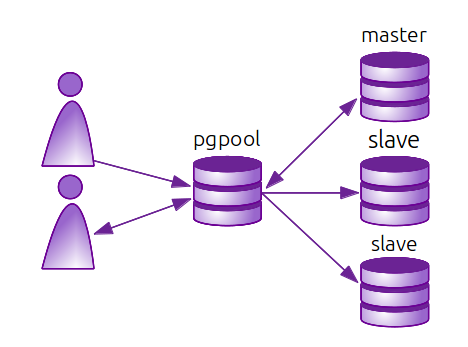
\includegraphics[scale=1]{../../../grafy/obr/schema_pgpool.png}
            \caption{Schéma pgpool}
            \label{pgpool_obr}
          \end{figure}

